\documentclass[blackandwhite]{beamer}

\mode<presentation>
{
  \usetheme{JuanLesPins}
  \usecolortheme{dolphin}
}

\usepackage[english]{babel}
\usepackage{subfigure}
\usepackage{xunicode}
\usepackage{xltxtra}
\usepackage{fontspec}
\setmainfont{Ubuntu}

\title
{Disease spreading on small-world networks}

\author
{J.Hofman}

\institute
{
 Department of Computational Science\\
 University of Amsterdam}

\pgfdeclareimage[height=0.8cm]{university-logo}{logo.png}
\logo{\pgfuseimage{university-logo}}

\begin{document}

\begin{frame}
  \titlepage
\end{frame}

\begin{frame}{Outline}
  \tableofcontents
\end{frame}


\section{Theory}

\subsection{Watts-Strogatz models}

\begin{frame}{Construction}
	\begin{itemize}
	\item
	Start with a regular ring graph of size $N$ where each node has $K$ neighbors, $K >> log(N)$, $K/2$ at each side.
	\item
	Rewire connections with probability $p$.
	\item
	$p = 0$: Completely structured graph.\\
	$p = 1$: Random graph.
	\end{itemize}
	\begin{center}
	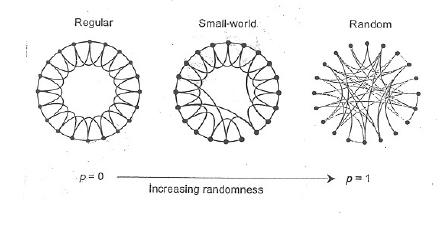
\includegraphics[scale=0.5]{smallworld.jpg}
	\end{center}
\end{frame}

\begin{frame}{Properties}
	\begin{itemize}
	\item
	Average path length L$(p,K)$: The average number of edges between two nodes in the graph.
	\item 
	Local clustering coefficient c$_{\text{i}}(p,K)$:\\
	\vspace{3mm}
	$\frac{\text{Number of connections between neighbors of node i}}{k(k-1)/2}$.
	\item
	Global clustering coefficient C$(p,K)$: $\frac{1}{N} \sum_{i = 1}^{N} $c$_{\text{i}}(p,K)$.
        \end{itemize}
        \begin{columns}[T]
        \column{.5\textwidth}
	\begin{center}
	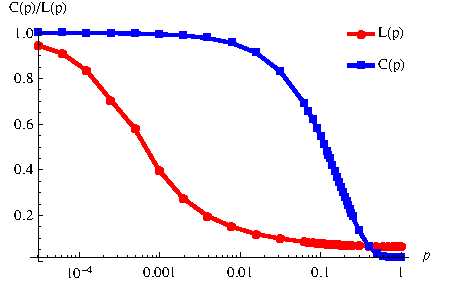
\includegraphics[scale=0.7]{lpcp.pdf}
	\end{center}
	\begin{itemize}
	\item
	In between: low L but high C $\Rightarrow$ small-world networks.
	\end{itemize}
        \column{.5\textwidth}
	small-world networks correspond to many realistic networks, e.g.:
	\begin{itemize}
	\item
	Social networks
	\item
	Neural networks
	\item
	Distributing networks (e.g. water and electric power grids)
	\end{itemize}
        \end{columns}
\end{frame}

\subsection{Disease models on networks}

\begin{frame}{SIR model}
	\begin{itemize}
	\item 
	Possible to simulate spreading of a disease on a network by means of assigning states to the nodes; the nodes represent people.
	\item 
	In this case three possible states: Susceptible (S), Infected (I), Recovered (R).
	\item
	Start with all nodes in S state except for one infected node. Infected node can infect neighbors with probability $p_{\text{inf}}$ every time step. Infected nodes change state to R and become inactive after $t_{\text{inf}}$ steps.
	\item
	Small example with $K = 3$, $N = 100$, $p_{\text{inf}} = 0.1$ and $t_{\text{rec}} = 5$: 
	\end{itemize}
\end{frame}

\begin{frame}{SIRS model}
	\begin{itemize}
	\item
	Same states as in the SIR model.
	\item
	Recovered nodes become susceptible again after $t_{\text{rec}}$.
	\item
	In contrast with SIR model this model does not have to reach a steady state.
	\end{itemize}
	Parameters used for both models:\\
	$N = 1000$\\
	$K = 5$\\
	$p_{\text{inf}} = 0.1$	 
\end{frame}


\section{Analysis}

\subsection{Infection rates}

\begin{frame}{Using SIR to determine infection spreading rate}
	\begin{itemize}
	\item
	Use SIR to determine the rate of disease spreading.
	\item
	$r_{1/2}$: the number of time steps before half of the population is infected.
	$r_{\text{tot}}$: the number of time steps before the total population is infected.
	\item
	$r_{\text{tot}}$ is only slightly bigger than $r_{1/2}$ for every $p$.\\
	Curves follow the same shape as L $\Rightarrow$ Disease spreading is fast on small-world networks.
	\end{itemize}
	\begin{center}
	\begin{figure}
	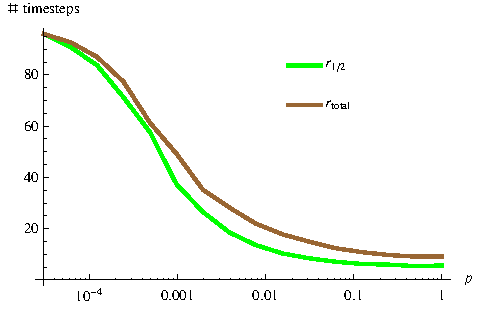
\includegraphics[scale=0.6]{r.pdf}
	\caption{$t_{\text{inf}} = 4$}
	\end{figure}
	\end{center}
\end{frame}

\subsection{Equilibrium states}

\begin{frame}{Reaching the equilibrium state}
	\begin{itemize}
	\item
	The SIRS model allows for investigation of a equilibrium state occurring afther the initial exponential infection rate.
	\item
	Behavior in equilibrium states very different for different values of $p$.
	\item
	Parameters used: $N = 1000$, $K = 5$, $p_{\text{inf}} = 0.1$, $t_{\text{inf}} = 8$, $t_{\text{rec}} = 8$.
	\end{itemize}
	\begin{figure}
	\subfigure[p = 2$^{-12}$]{
	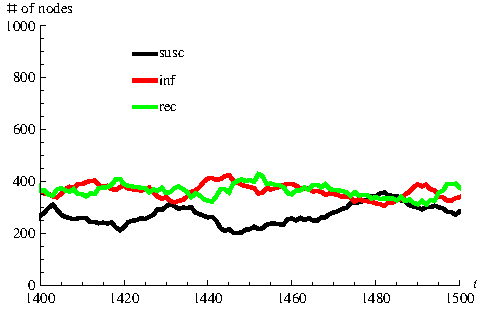
\includegraphics[scale=0.3]{periodlowp.pdf}
	}
	\subfigure[p = 2$^{-5}$]{
	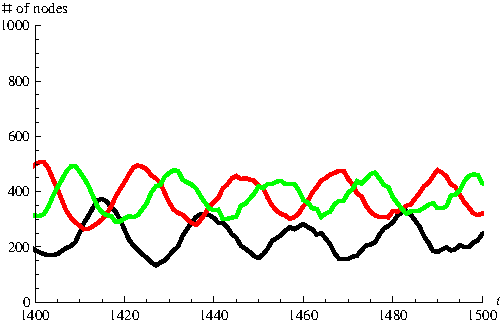
\includegraphics[scale=0.3]{periodmidp.pdf}
	}
	\subfigure[p = 1]{
	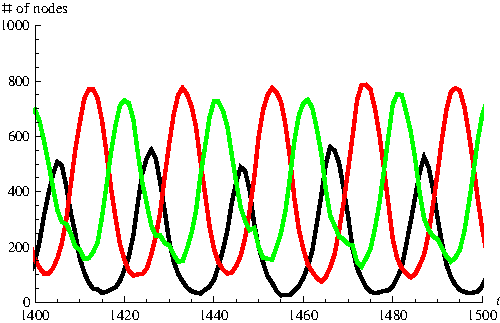
\includegraphics[scale=0.3]{periodhighp.pdf}
	}
	\end{figure}
	\begin{itemize}
	\item
	Period $\approx$ $t_{\text{inf}} + t_{\text{rec}} + 2$.
	\item
	There seems to occur a phase transition: unsynchronized states for low $p$ ; synchronized states for high $p$.
	\end{itemize}	
\end{frame}

\begin{frame}{The order parameter}
	\begin{itemize}
	\item
	Capture measure of synchronization in the order parameter: $\sigma (t) = \mid \frac{1}{N} \sum_{i = 1}^{N} e^{i \phi_{i} (t)} \mid$ with $\phi_{i} (t) = 2 \pi \frac{\tau_{i} - 1}{t_{\text{inf}} + t_{\text{rec}}}$.
	\item
	Leave out states with $\tau = 0$ for a clearer signal.
	\end{itemize}
	\begin{center}
	\begin{figure}
	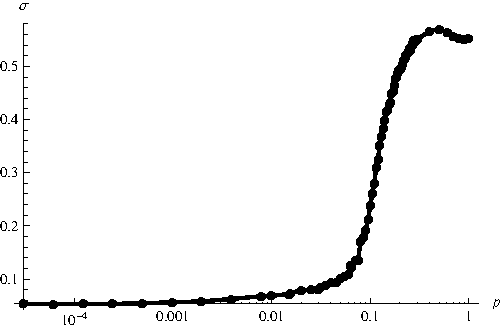
\includegraphics[scale=0.5]{sigma.pdf}
	\end{figure}
	\end{center}
\end{frame}

\begin{frame}
	\begin{itemize}
	\item
	The derivative of $\sigma$ is largest when the derivative of C$(p)$ is largest.
	\item
	Look at the standard deviation of c$_{i}(p)$.
	\item
	Large standard deviation means large spreading in the amount of clustering.
	\item
	Peak of standard deviation coincides with derivative of $\sigma$.
	\end{itemize} 
	\begin{center}
	\begin{figure}
	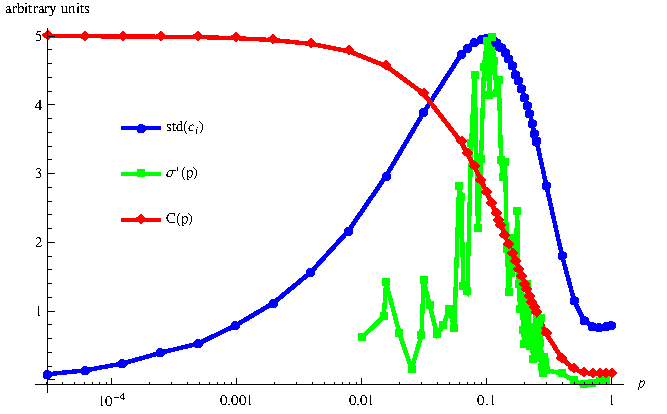
\includegraphics[scale=0.5]{std.pdf}
	\end{figure}
	\end{center}
\end{frame}

\section{Conclusion and discussion}

\subsection{Conclusion}

\begin{frame}
	\begin{itemize}
	\item
	Small-networks have properties that coincide with many real life networks.
	\item
	Spreading of diseases on networks scales with L$(p)$.
	\item
	Synchronization of states occurs at high values of $p$, onset of synchronization seems to be coupled with decreasing C($p$) and large $\sigma(\text{c}_{i}(p))$.
	\end{itemize}
\end{frame}

\subsection{Discussion}

\begin{frame}
	\begin{itemize}
	\item
	Static edges not always very realistic; use dynamic models.
	\item
	Outcome highly dependent on $N$, $K$, $p_{\text{inf}}$, $t_{\text{inf}}$ and $t_{\text{rec}}$, in reality possibly all functions of $t$.
	\item
	Model does not take into account behavioral aspects of people.
	\item
	Analytical background of small-world networks still poorly understood.
	\end{itemize}
\end{frame}

\begin{frame}
  \tiny
  Software:
  \begin{itemize}
  \item
  PYTHON: coding
  \item
  IGRAPH: package for manipulatin, constructing and plotting/animating graphs.
  \item
  NUMPY: package for linear algebra in Python.
  \item
  Mathematica: graphical output and basic manipulations.
  \end{itemize}
  References:
  \begin{itemize}
  \item
  Watts, Duncan J.; Strogatz, Steven H.., \emph{Collective dynamics of 'small-world' networks}, Nature, 6/4/98, Vol. 393 Issue 6684, p440
  \item
  Kuperman, M.; Abramson, G.,\emph{Small World Effect in an Epidemiological Model}, Phys. Rev. Letters, 3/2001, Vol. 86, p2909-2912, [arXiv:nlin/0010012]
  \item
  Li, Sheng; Meng, Meng; Ma, Hongru,\emph{Epidemic Spreading in Dynamic Small World Networks}, [arXiv:nlin/0411017]
  \item
  Bollabas, B., \emph{Random Graphs}, Academic, London, 1985.
  \item
  Y. Kuramoto, \emph{Chemical Oscillations, Waves, and Turbu-
lence}, Springer, Berlin, 1984.
  \end{itemize}
\end{frame}
\end{document}


